The following is a brief description of HMMs adapted from \cite{mesa2016hidden}. 

Let $x = (x_1,x_2,\ldots,x_n)$ be a sequence of observations, also known as emissions or residues, where each $x_j$ takes values from a finite alphabet $D$. 
Also $y = (y_1,y_2,\ldots,y_n)$ is a collection of states, where each $y_i$ belongs to $\mathcal{E}$, a finite set of states. In application, these states may correspond to different classes of genomic element; for example, intergenic regions, TFBSs, introns or exons. The sequence $x$ can be thought of as a time series where the indices $j$ are taken as discrete time steps. These models are considered 'hidden' because only sequence of residues $x$ is observable and but the sequence of states $y$ is unknown.
 
    \begin{figure}[H]
        \centering
        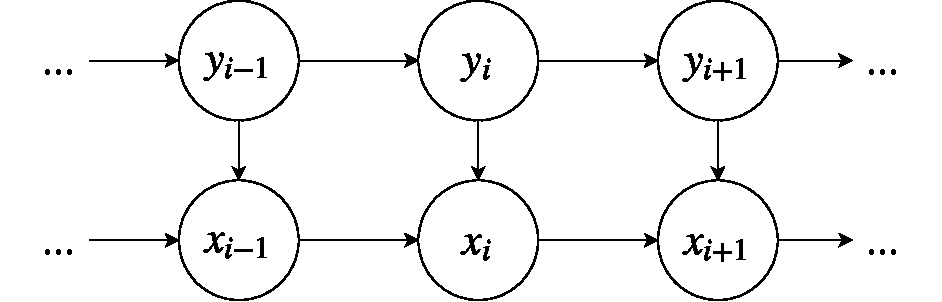
\includegraphics[width=0.6\textwidth]{HMM.pdf}
        \caption{A schematic of the unknown sequence of states $y$ generating the observed sequence $x$.}
        \label{fig:HMM}
    \end{figure}
The model assumption is that the sequence $x$ is generated by starting at some initial state $y_1$, produces a residue $x_1$ and moves to a new state and produces a new residue. This continues until the end of the sequence (see Figure~\ref{fig:HMM}). Let $P(x_i|y_i = k)$ denote the probability that the emission $x_i$ was produced by state $k$ at step $i$. Next, let the probability that a transition is made from state $k$ to state $l$ given by $P(y_{i+1} = l | y_i = k)$. The joint distribution for the probability the model transits path $y$ and generates the sequence $x$ is then
	\begin{equation}
		P(x,y) = \prod_{i=1}^{n} P(y_i|y_{i-1})P(x_i|y_i),
	\end{equation}
where $P(y_i|y_{i-1}) = P(y_{i} = l | y_{i-1} = k)$ and $P(x_i|y_i) = P(x_i|y_i = k)$. 

The parameters of the model are the state transition probabilities and the emission probabilities for each state. In practice, these parameters are estimated for example with Expectation Maximisation.

There are three assumptions underlying the model:
	\begin{itemize}
		\item The Markov property holds for the states $y_i$. That is $P(y_{i+1}|y_i,\ldots,y_1) = P(y_i|y_{i-1})$.
		\item The Markov chain produced by the states $y$ is homogeneous. That is the probability of transitioning from one state to another is independent of time $i$. 
		\item Conditional independence of observations. That is $x_i$ is only dependant on the state $y_i$. 
	\end{itemize}

An example of usage would be to assign the alphabet $D = \{A,C,G,T\}$ representing the four nucleotide bases found in DNA or $D$ being some alphabet that is able to encode information about the epigenetic status of the DNA and for the states as $\mathcal{E} = \{\text{intron}, \text{exon}, \text{intergenic region}\}$. 
% These models have been used in computational biology \textbf{cite?}

%albus, silas, salus, meris, janus, miles, myles, regis, remus  





